\section{Error Introduced by Linear Interpolation}
We obtain the initial conditions for the standing accretion shock problem with an external code. We then have to interpolate these data onto the grid for use in \texttt{thornado}. We start by proving that linear interpolation is a convex combination of the solution at the boundary points.

\subsection{Proof that Linear Interpolation is a Convex Combination of Boundary-Points}
Linear interpolation of a function, $f$, of a variable, $r$, bounded by two points $r_{L}$ and $r_{H}$, with $r_{H}>r_{L}$, can be written as:
\begin{equation}
    f\left(r\right)=f\left(r_{L}\right)+\f{f\left(r_{H}\right)-f\left(r_{L}\right)}{r_{H}-r_{L}}\left(r-r_{L}\right).
\end{equation}
By making a change of variables from $r$ to $\eta$, where:
\begin{equation}
    r\left(\eta\right)=\eta\,r_{H}+\left(1-\eta\right)r_{L}=r_{L}+\eta\,\Delta r\implies\eta=\f{r-r_{L}}{\Delta r},\hspace{1em}\eta\in\left[0,1\right],
\end{equation}
such that $r\left(\eta=0\right)=r_{L}$ and $r\left(\eta=1\right)=r_{H}$, we have that:
\begin{align}
    f\left(\eta\right)&=f\left(0\right)+\f{f\left(1\right)-f\left(0\right)}{1-0}\left(\eta-0\right)=f\left(0\right)+\left(f\left(1\right)-f\left(0\right)\right)\eta\\
    \implies f\left(\eta\right)&=\eta\,f\left(1\right)+\left(1-\eta\right)f\left(0\right).
\end{align}

So when we interpolate a fluid variable, say the mass-density $\rho$, we have:
\begin{equation}
    \rho\left(r\right)=\rho_{L}+\f{\Delta\rho}{\Delta r}\left(r-r_{L}\right)\longrightarrow\rho\left(\eta\right)=\eta\,\rho_{H}+\left(1-\eta\right)\rho_{L},
\end{equation}
where $\rho_{L}\equiv\rho\left(r_{L}\right)$ and $\rho_{H}=\rho\left(r_{H}\right)$.


\subsection{Example: $f\left(x\right)=x^{2}$}
We can show this directly for simple functions. We take as an example $f\left(x\right)=x^{2}$:
\begin{align}
    f\left(x\right)&=x^{2}=\left[x_{L}+\eta\left(x_{R}-x_{L}\right)\right]^{2}=x_{L}^{2}+\eta^{2}\left(x_{R}-x_{L}\right)^{2}+2\,x_{L}\,\eta\left(x_{R}-x_{L}\right)\\
    &=x_{L}^{2}+\eta^{2}\,x_{R}^{2}+\eta^{2}\,x_{L}^{2}-2\,\eta^{2}\,x_{L}\,x_{R}+2\,\eta\,x_{L}\,x_{R}-2\,\eta\,x_{L}^{2}.
\end{align}
Now we add and subtract the interpolated solution: $\eta\,x_{H}^{2}+\left(1-\eta\right)x_{L}^{2}$. This yields:
\begin{align}
    x^{2}&=x_{L}^{2}+\eta^{2}\,x_{R}^{2}+\eta^{2}\,x_{L}^{2}-2\,\eta^{2}\,x_{L}\,x_{R}+2\,\eta\,x_{L}\,x_{R}-2\,\eta\,x_{L}^{2}+\eta\,x_{H}^{2}+\left(1-\eta\right)x_{L}^{2}-\eta\,x_{H}^{2}-\left(1-\eta\right)x_{L}^{2}\\
    &=\left[\eta\,x_{H}^{2}+\left(1-\eta\right)x_{L}^{2}\right]+\left[-\eta\left(1-\eta\right)x_{L}^{2}-\eta\left(1-\eta\right)x_{H}^{2}+2\,\eta\,x_{L}\,x_{H}\left(1-\eta\right)\right]\\
    &=\left[\eta\,x_{H}^{2}+\left(1-\eta\right)x_{L}^{2}\right]-\eta\left(1-\eta\right)\left[x_{L}^{2}+x_{H}^{2}-2\,x_{L}\,x_{H}\right]\\
    &=\left[\eta\,x_{H}^{2}+\left(1-\eta\right)x_{L}^{2}\right]-\eta\left(1-\eta\right)\left(x_{H}-x_{L}\right)^{2}\\
    &=\left[\eta\,x_{H}^{2}+\left(1-\eta\right)x_{L}^{2}\right]-\eta\left(1-\eta\right)\left(\Delta x\right)^{2}.
\end{align}
The term in square brackets is the interpolated solution, and the second term is the remainder, i.e. the error in the interpolated solution. So we see that when using linear interpolation to interpolate the function $f\left(x\right)=x^{2}$ we introduce an error (of the order $\left(\Delta x\right)^{2}$) that goes to zero as the step-size goes to zero.

As a final step we replace $\eta$ with $x$, yielding:
\begin{align}
    f\left(x\right)=x^{2}&=x_{L}^{2}+\f{x_{H}^{2}-x_{L}^{2}}{x_{H}-x_{L}}\left(x-x_{L}\right)-\left(x-x_{L}\right)\left(x_{H}-x\right)\\
    &=f\left(x_{L}\right)+\f{\Delta f}{\Delta x}\left(x-x_{L}\right)-\left(x-x_{L}\right)\left(x_{H}-x\right).
\end{align}

We show the results of this in the following figure:
\begin{figure}[H]
\centering
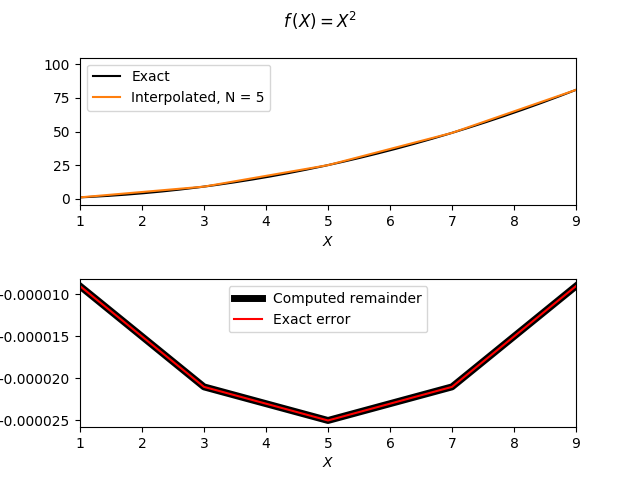
\includegraphics[scale=0.75]{LinearInterpolationError}
\end{figure}

\subsection{Mass Constant}
The mass constant, $C_{D}$, from the 3+1 GR hydrodynamics equations is:
\begin{equation}
    C_{D}\left(r\right)=\psi\left(r\right)^{6}\,\alpha\left(r\right)\,r^{2}\,\rho\left(r\right)\,W\left[v\left(r\right)\right]\,v\left(r\right).
\end{equation}
When we map from the radial coordinates from the original data to the mesh in \texttt{thornado} we don't introduce any error, because it is a linear map. This means that all the error we introduce must be due to $\rho$, $W$, and $v$. So, when deriving the error we consider the different function:
\begin{equation}
    C'_{D}\left(r\right)\equiv\f{C_{D}\left(r\right)}{\psi\left(r\right)^{6}\,\alpha\left(r\right)\,r^{2}}=\rho\left(r\right)\,W\left[v\left(r\right)\right]\,v\left(r\right).
\end{equation}

From the data we have this exact value at the two endpoints:
\begin{align}
    C'_{D}\left(r_{L}\right)&\equiv C'^{L}_{D}=\rho_{L}\,W_{L}\,v_{L}\\
    C'_{D}\left(r_{H}\right)&\equiv C'^{H}_{D}=\rho_{H}\,W_{H}\,v_{H}.
\end{align}
